\documentclass{article}

\usepackage{times}
\usepackage{geometry}
\geometry{a4paper,left=0.6cm,right=0.7cm,top=2cm,bottom=1cm,columnsep=0.8cm}
\usepackage{fontawesome}
\usepackage[hidelinks]{hyperref}
\usepackage{multicol}
\usepackage{tikz}
\usepackage{hyphsubst}
\usepackage{moresize}
\usepackage{hyphenat}
\usepackage{tabularx}
\usepackage{xcolor}
\usepackage{enumitem}
\usetikzlibrary{calc, positioning}      
\newcolumntype{Y}{>{\RaggedRight\arraybackslash}X}

% Définition des couleurs
\definecolor{maincolor}{HTML}{f0fafc}
\definecolor{seccolor}{HTML}{ffffff}
\definecolor{gray}{HTML}{8c94a9}
\definecolor{sidetext}{HTML}{59cee5}

% Solution robuste pour la bande bleue sur toute la hauteur
\usepackage{eso-pic}
\AddToShipoutPictureBG{%
  \begin{tikzpicture}[remember picture,overlay]
    \fill[maincolor] 
        (current page.north west) rectangle 
        ([xshift=0.3\paperwidth] current page.south west);
  \end{tikzpicture}%
}

% Configuration des listes
\setlist[itemize]{itemsep=-2pt,topsep=0pt,leftmargin=1.08cm}
\renewcommand{\labelitemi}{\textcolor{sidetext}{\footnotesize$\bullet$}}

\setlength{\parindent}{0pt}
\usepackage{paracol}
\columnratio{0.3}

\begin{document}

\pagestyle{empty}

\begin{paracol}{2}
% ----------------------------------------------------------------
% Colonne gauche - Informations personnelles
% ----------------------------------------------------------------
\color{sidetext}
\begin{center}
    \begin{tikzpicture}
        \clip (0,0) circle (1.5cm) node[anchor=center] {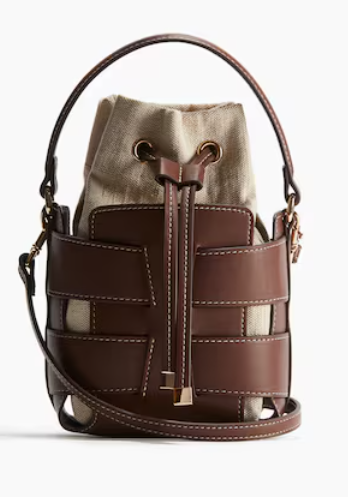
\includegraphics[width=3cm]{30107c79b2a646cd97dea8cad4d7537a.png}}; 
    \end{tikzpicture}

    \vspace{5mm}
    
    {\color{black}\LARGE \textbf{Dora SARKIS}}
    
    \vspace{3mm}
    
    {\large{Gérante \& Directrice d'Événements}}
\end{center}

{\color{gray}\rule{\linewidth}{0.4pt}} \\

% ------------------ Coordonnées ------------------
\begin{tabular}{@{}c l}
    \faPhone{} & 
    \begin{tabular}[t]{@{}l@{}}
        {\color{gray}Téléphone} \\
        06\,90\,59\,69\,69
    \end{tabular} \\
    \\
    \faMapMarker{} & 
    \begin{tabular}[t]{@{}l@{}}
        {\color{gray}Adresse} \\
        53 résidence Les Citronnelles
    \end{tabular} \\
    \\
    \faEnvelope{} & 
    \begin{tabular}[t]{@{}l@{}}
        {\color{gray}Mail} \\
        leroyalriviera@gmail.com
    \end{tabular} \\
\end{tabular}

\vspace{3mm}
{\color{gray}\rule{\linewidth}{0.4pt}} \\

% ------------------ Compétences ------------------
\vspace{5mm}
{\color{black}{Compétences Clés}}

\vspace{5mm}

\begin{tabular}{@{}c l}
    \textcolor{sidetext}{\faBuilding} & Gestion d’entreprise \\
    \\
    \textcolor{sidetext}{\faHandshakeO} & Négociation commerciale \\
    \\
    \textcolor{sidetext}{\faUsers} & Relation client \\
    \\
    \textcolor{sidetext}{\faCalendarCheckO} & Organisation d’événements \\
    \\
    \textcolor{sidetext}{\faBriefcase} & Management \& gestion administrative \\
    \\
    \textcolor{sidetext}{\faCheckCircle} & Autonomie, rigueur, sens de l’organisation \\
\end{tabular}

% ------------------ Centres d’intérêt ------------------
\vspace{5mm}
{\color{black}{Centres d’intérêt}}

\vspace{5mm}

\begin{tabular}{@{}c l}
    \textcolor{sidetext}{\faBalanceScale} & Droit commercial, des affaires et immobilier \\
\end{tabular}

% Espace flexible pour étendre la colonne gauche
\vfill
~

% ----------------------------------------------------------------
\switchcolumn
% ----------------------------------------------------------------
\color{black}

% ------------------ Profil ------------------
\textcolor{black}{\Large \textbf{Profil Professionnel}} \\

Entrepreneure passionnée depuis 2008, j’ai fondé et dirigé plusieurs structures dédiées à l’organisation d’événements et à la vente spécialisée. Mon parcours m’a permis d’acquérir une solide expérience en gestion d’entreprise, management d’équipes et négociation commerciale. Rigoureuse et autonome, j’excelle dans le développement d’offres orientées client et dans la coordination d’activités administratives complexes. Je recherche de nouveaux défis pour mettre à profit mes compétences de leadership et d’organisation d’événements.\\[8pt]

% ------------------ Expérience professionnelle ------------------
\textcolor{black}{\Large \textbf{Expérience Professionnelle}} \\

% ---- Expérience 1 ----
\colorbox{maincolor}{%
  \begin{minipage}{\linewidth}
    \begin{tabular}{@{}l l r}
        \textcolor{sidetext}{\faBriefcase} & 
        \textbf{Gérante} &  
        \footnotesize{2019 -- Présent} \\
        & \textit{Boutique \& gestion de locaux commerciaux, Pointe-à-Pitre} & \\
    \end{tabular}
    \begin{itemize}
        \item Supervision quotidienne de la boutique et administration de plusieurs locaux commerciaux. 
        \item Gestion globale : développement de l’offre, négociation fournisseurs et relation client sur site. 
        \item Pilotage des obligations administratives et financières avec autonomie et rigueur.
    \end{itemize}
  \end{minipage}%
}

\vspace{5mm}

% ---- Expérience 2 ----
\colorbox{maincolor}{%
  \begin{minipage}{\linewidth}
    \begin{tabular}{@{}l l r}
        \textcolor{sidetext}{\faBriefcase} & 
        \textbf{Directrice} &  
        \footnotesize{2012 -- 2018} \\
        & \textit{Salle de spectacle} & \\
    \end{tabular}
    \begin{itemize}
        \item Management complet de la structure : équipe, programmation et logistique d’événements. 
        \item Organisation opérationnelle et suivi administratif, assurant la rentabilité de la salle. 
        \item Mise en place de procédures optimisant la gestion financière et la satisfaction des clients.
    \end{itemize}
  \end{minipage}%
}

\vspace{5mm}

% ---- Expérience 3 ----
\colorbox{maincolor}{%
  \begin{minipage}{\linewidth}
    \begin{tabular}{@{}l l r}
        \textcolor{sidetext}{\faBriefcase} & 
        \textbf{Gérante fondatrice} &  
        \footnotesize{2008} \\
        & \textit{Joykiss – Boutique mariage \& wedding planning} & \\
    \end{tabular}
    \begin{itemize}
        \item Création et développement d’une offre spécialisée mariage, incluant services de wedding planning et design. 
        \item Gestion commerciale et relation client, du premier contact jusqu’à la signature. 
        \item Négociation avec partenaires et fournisseurs afin de maximiser la valeur ajoutée pour les clients.
    \end{itemize}
  \end{minipage}%
}

\vspace{8mm}

% ------------------ Formation ------------------
\textcolor{black}{\Large \textbf{Formation}} \\

% ---- Formation 1 ----
\begin{tabular}{@{}c l}
    \textcolor{sidetext}{\faGraduationCap} & 
    \begin{tabular}[t]{@{}l@{}}
        \textbf{Formation en décoration événementielle} \\
        Centre ABC \\
        Approche pratique de la scénographie et du design d’événements. \\
        2008
    \end{tabular} \\
\end{tabular}

\vspace{5mm}

% ---- Formation 2 ----
\begin{tabular}{@{}c l}
    \textcolor{sidetext}{\faGraduationCap} & 
    \begin{tabular}[t]{@{}l@{}}
        \textbf{BTS Commerce international (inachevé)} \\
        CNED \\
        Programme axé sur les techniques de négociation et la gestion des échanges mondiaux. \\
        2008
    \end{tabular} \\
\end{tabular}

\vspace{5mm}

% ---- Formation 3 ----
\begin{tabular}{@{}c l}
    \textcolor{sidetext}{\faGraduationCap} & 
    \begin{tabular}[t]{@{}l@{}}
        \textbf{Baccalauréat professionnel Commerce} \\
        CNED \\
        Formation orientée vente, gestion de clientèle et techniques commerciales. \\
        2006
    \end{tabular} \\
\end{tabular}

\vspace{8mm}
\end{paracol}

\end{document}